\subsection{Competition results$^\odot$}
The competition took place on two dates (15th and 17th of September) and each team had to play three simulations against all other teams.
Every simulation consisted of a total of 400 steps.
The team with the higher overall score at the end received three points for their victory.
Said overall score is the sum of all 400 step scores.
The score per step is composed of points for zones plus achievement points.
Since the strategy of team MAKo was to extensively buy upgrades for the so-called artillery agent, most of the earned achievement points were consumed and therefore did not count towards the step score.
Figure \autoref{dis:achievement_points} shows the progress of achievement points over time.
As can be seen, the achievement points of team MAKo go up and down due to the buying actions whereas the the points of the other team increase constantly.
\begin{figure}[ht]
	\centering
	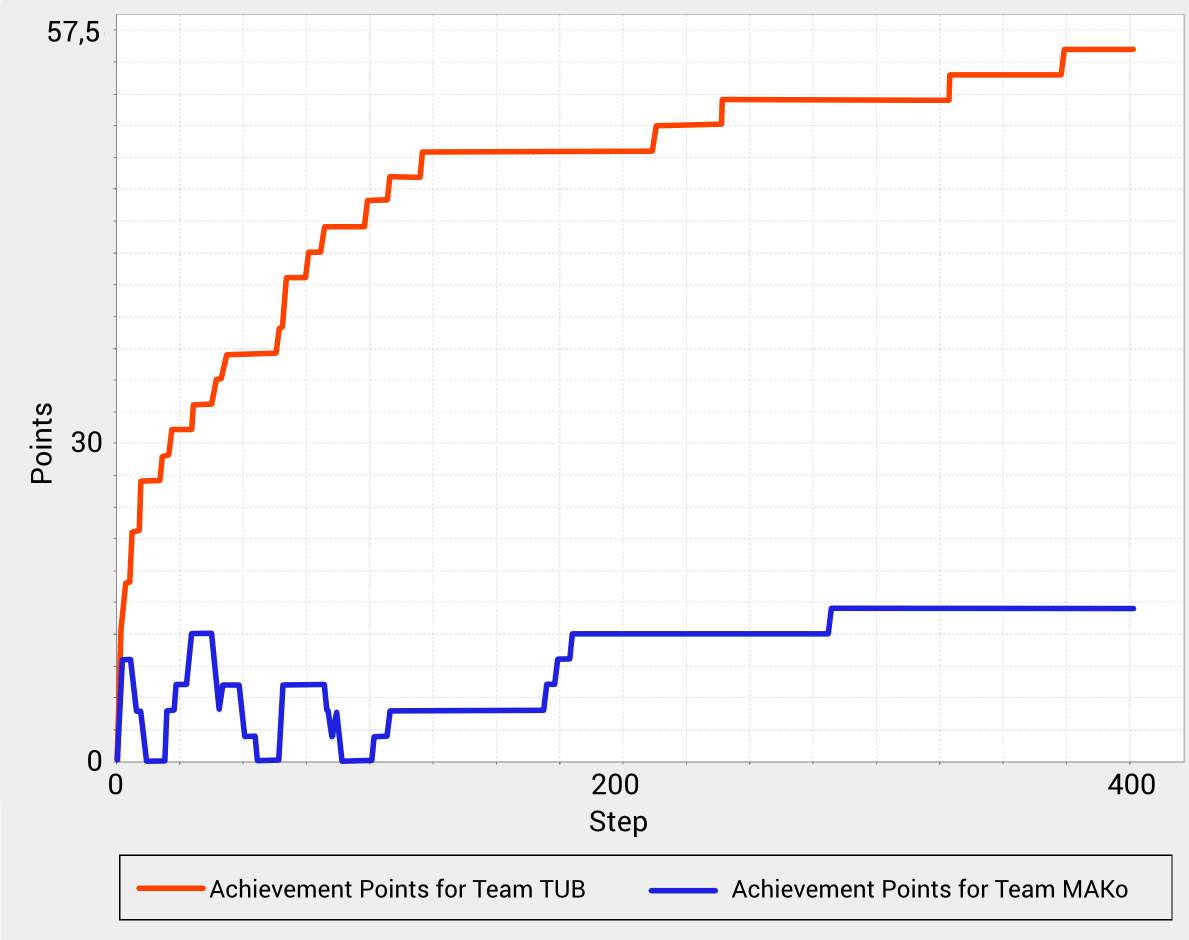
\includegraphics[width=\textwidth]{images/AchievementPoints.png}
	\caption{Achievement points from the second match TUB against MAKo.} % TODO I just wrote second as a filler. What match was it?
	\label{dis:achievement_points}
\end{figure}
On first sight, one could assume that this strategy was a drawback because achievement points earned at some point count into every future step score.
But compared to the number of points awarded for zones, the achievement points are only a minor fraction of the step score.
As it can be seen in \autoref{dis:ZonesScoresAndAchievementPoints} the spending of achievement points did not interfere dramatically with the overall score.
It was worth spending the achievement points for the purpose of attacking and disturbing the other team.
This was because the amount of potential zone points they would have earned without being attacked, would probably have been much higher than the amount of achievement points team MAKo spent for upgrades.
\begin{figure}[h]
	\centering
	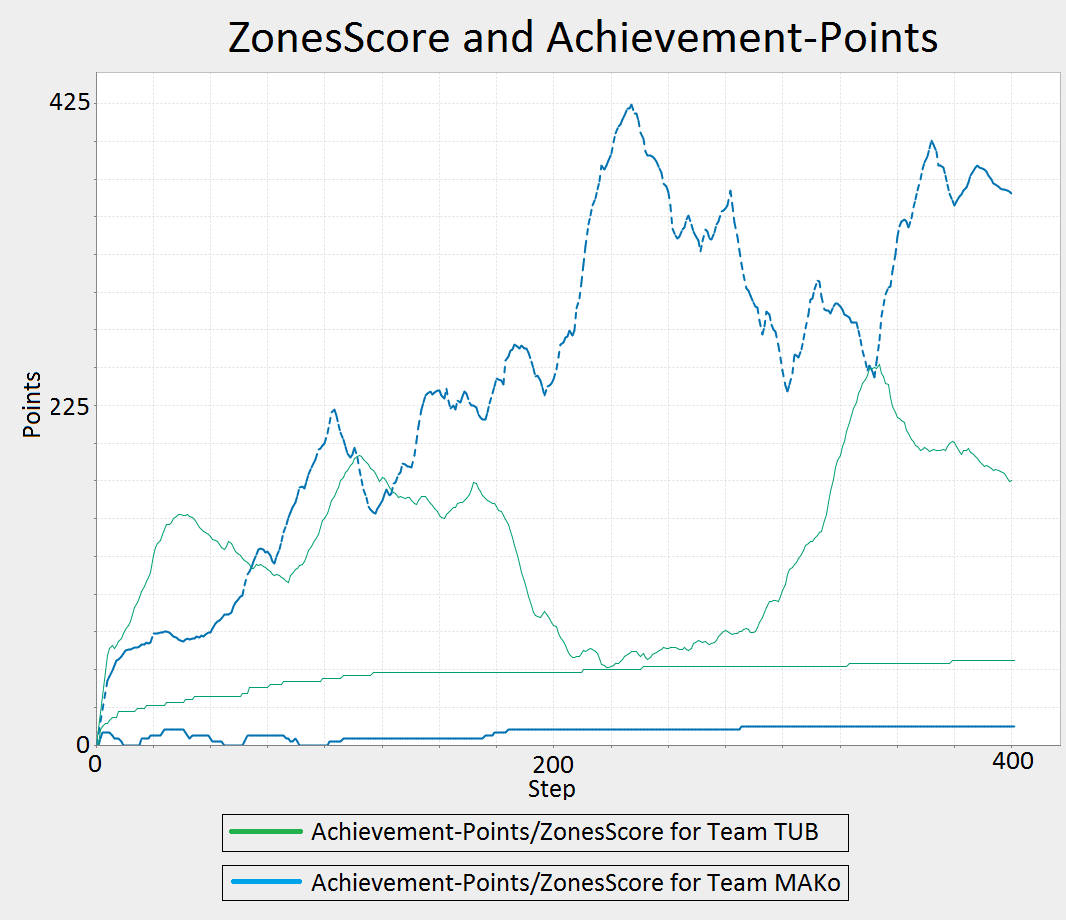
\includegraphics[width=\textwidth]{images/ZonesScoresAndAchievementPoints.png}
	\caption{Combined achievement and zone scores from the second match TUB against MAKo.} % TODO I just wrote second as a filler. What match was it?
	\label{dis:ZonesScoresAndAchievementPoints}
\end{figure}
At the end of the tournament team MAKo scored second with a total of 18 points.
The winner of 2014 was, for the third time in a row now, the team from the USFC.
The final results are shown in~\autoref{tab:mapc2014results}.
\begin{table}[ht]
\centering
\caption{The results of the 2014 MAPC. Each team played three matches against every other team, and winning a match awarded 3 points.}
\label{tab:mapc2014results}
\begin{tabular}{@{}lllll@{}}
\toprule
Pos. & Team name      & Score            & Difference            & Points \\ \midrule
1    & SMADAS-UFSC    & 1180662 : 654624 & \phantom{-}526038     & 33     \\
2    & MAKo           & 617086 : 776868  & -15782                & 18     \\
3    & TUB            & 904874 : 872399  & \phantom{-}32475      & 15     \\
4    & TheWonderbolts & 711001 : 1014669 & -303668               & 15     \\
5    & GOAL-DTU       & 653178 : 748241  & -95063                & 9      \\ \bottomrule
\end{tabular}
\end{table}
Statistics of all the individual games can be found in the appendix.[reference here!!!!]

Team MAKo lost every second game against each opponent due to the fact that for some reason the repairer agents weren't able to repair. The reason behind this was not obvious to the team. Summarizing the matches, team MAKo was capable of exploring the map, building local optima zones, dealing with disabled agents and attacking the opponent. A thing that could be improved is the zoning behaviour. Due to the fact that zones were broken up on a regular basis, zones with a high value sometimes were discarded even when there was no need to do that. Also no handling of edge cases has been implemented which could improve zoning in the sense that the actual number of agents needed to build that zone could be less than the number calculated by our algorithm. But the general idea regarding small zone forming was good. Because one big zone is easy to disturb, having some small high value zones was quite effective to not provide the enemy with an easy target. Like already mentioned a strategy that worked out well, was the approach to upgrade the visibility range and the strength of one saboteur agent significantly. In all matches the it was able to disable enemy agents many times and therefore disturb zones and keep the enemy repairers busy, which kept them away from building zones.

% TODO: these are from the TOC:
%What place did we rank? How did the others do? Analyse our matches shortly and point out problems we faced, how we tackled them and point out what had gone well.
